\documentclass[11pt,a4paper]{article}
 
\usepackage[brazilian]{babel}
\usepackage[utf8]{inputenc}
\usepackage{graphicx}
\usepackage{subfigure}
\usepackage[numbered,framed]{mcode}
\usepackage{amsmath}
\hyphenation{}
\graphicspath{{img/}}

\title{ITVsim - Manual do Usuário}
\date{}

\begin{document}
\maketitle
\tableofcontents

\section{Introdução} 
\textit{ITVsim} é um simulador de estratégias cooperativas para
múltiplos rôbos aéreos desenvolvido para o projeto
\textit{Desenvolvimento de Veículos Autônomos Cooperativos para
  Mapeamento e Mineração}. O principal objetivo do sistema é
disponibilizar um ambiente de desenvolvimento prático com foco em
interações simples entre os robôs e o ambiente, de modo que o usuário
apenas se preocupe com os comportamentos de alto nível contidos na
estratégia de cooperação. Para tanto, os modelos físicos e a
comunicação entre os robôs são extremamente simplificados e não
condizem com as restrições existentes em sistemas reais. Dessa
maneira, o uso do sistema é indicado durante as primeiras etapas do
projeto, quando a estratégia de cooperação está em processo de
definição, podendo ser testada com um número arbitrário de robôs e
comparada com outras estratégias candidatas. Para simulações
complexas, é recomendado o uso do \textit{Robot Operating System}
(http://www.ros.org/) em conjunto com o simulador Gazebo
(http://gazebosim.org/).

O simulador \textit{ITVsim} foi desenvolvido no ambiente
\textit{MATLAB R2013a} devido às facilidades envolvidas na programação
de controladores por parte do usuário. Além disso, como os modelos
físicos e de comunicação são simplificados, o sistema não requer uma
capacidade elevada de processamento, o que justifica a utilização de
uma linguagem de programação de alto nível.


\section{Interface}
Na Figura \ref{fig:principal} é apresentada a interface principal do
\textit{ITVsim}, que é dividida em cinco subinterfaces: visualizador,
mapa de anomalias, configurações do terreno, da simulação e do
renderizador.

\begin{figure}[htpb]
  \centering
  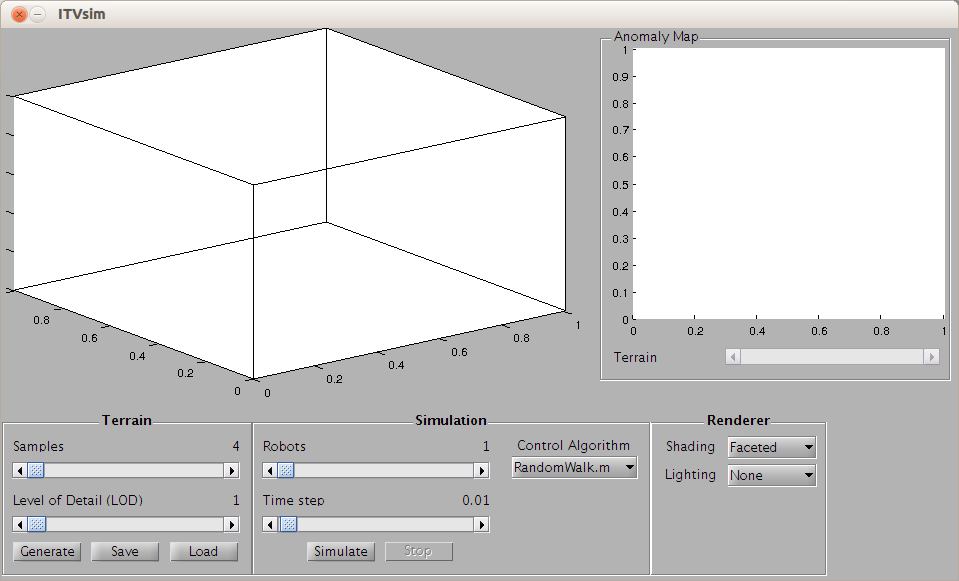
\includegraphics[width=\textwidth]{ITVsim.png}
  \caption{Interface principal do \textit{ITVsim}.}
  \label{fig:principal}
\end{figure}

\subsection{Visualizador}
\label{sec:visualizer}

O visualizador representa a simulação graficamente para o usuário,
como mostrado na Figura \ref{fig:visualizer}. Existem três elementos
gráficos contidos na simulação: o terreno, o mapa de anomalias e os
robôs. O terreno é caracterizado por uma grade regular de vértices
cujas alturas seguem a topografia de um modelo analítico interno do
simulador, mas um arquivo externo com dados reais também pode ser
utilizado. O mapa de anomalias encontra-se abaixo do terreno e
representa as anomalias magnéticas contidas no mesmo através de um
gradiente ciano--magenta. Os robôs são representados como círculos
vermelhos. Todos os elementos gráficos são renderiados através de uma
projeção ortográfica.

\begin{figure}[htpb]
  \centering
  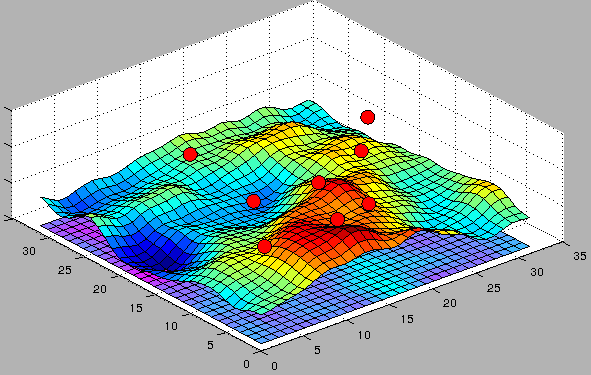
\includegraphics[width=\textwidth]{visualizer.png}
  \caption{Elementos gráficos do Visualizador.}
  \label{fig:visualizer}
\end{figure}

Em termos de interação, o usuário pode rotacionar a cena clicando com
o botão esquerdo do mouse e o arrastando em qualquer direção. Além
disso, o botão direito permite acessar um menu que contém diversas
opções de visualização, tais como:

\begin{itemize}
\item\textbf{ Reset to Original View}: retorna o visualizador às
  configurações iniciais do simulador.
\item \textbf{Goto X-Y view}: rotaciona a cena para visualização no
  plano X-Y.
\item \textbf{Goto X-Z view}: rotaciona a cena para visualização no
  plano X-Z.
\item \textbf{Goto Y-Z view}: rotaciona a cena para visualização no
  plano Y-Z.
\item \textbf{Plot box rotate}: desabilita o modo de rotação com
  renderização contínua (recomendado para computadores com baixo
  processamento).
\item \textbf{Continuous rotate}: habilita o modo de rotação com
  renderização contínua.
\item \textbf{Stretch-to-fill axes}: Estende os eixos X-Y para cobrir
  todo o espaço livre do visualizador.
\item \textbf{Fixed aspect ratio axes}: Mantém a mesma proporção nos
  eixos X-Y do visualizador.
\end{itemize}

\subsection{Mapa de Anomalias}
O mapa de anomalias é criado através de um modelo analítico interno do
simulador e \textbf{não representa um modelo real de anomalias
  magnéticas}. Como o foco do \textit{ITVsim} é o algoritmo de
cooperação, métricas como a razão entre a área coberta e o tempo se
sobrepõem à veracidade dos dados coletados. Assim, o objetivo do mapa
de anomalias é apenas prover uma visualização da cobertura relacionada
com a estratégia desenvolvida.

Além da representação contida no visualizador (Seção
\ref{sec:visualizer}), o \textit{ITVsim} provê a o mapa de anomalias
em visão aérea, tanto globalmente quanto localmente, isto é, em
relação ao conhecimento de cada robô
(Figura~\ref{fig:anomalies}). Esses mapas podem ser acessados
individualmente através da barra de rolagem vertical localizada logo
abaixo da representação gráfica dos mesmos. Com relação aos mapas
locais, as células em vermelho escuro (Figura \ref{fig:anomalies_b})
representam informações desconhecidas pelo robô.

\begin{figure}[htpb]
  \centering
  \subfigure[Mapa global.]{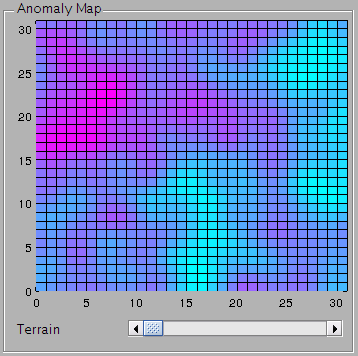
\includegraphics[width=0.45\textwidth]{anomalymap-1.png}} 
  \subfigure[Mapa local.]{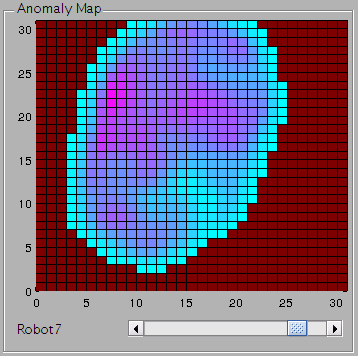
\includegraphics[width=0.45\textwidth]{anomalymap-2.png} \label{fig:anomalies_b}}
  \caption{Visualizações aéreas do mapa de anomalias global e local.}
  \label{fig:anomalies}
\end{figure}

A leitura do mapa local é feita em cada iteração através um cone com
ápice na posição do robô. Desse modo, quanto maior a altura do robô em
relação ao terreno, maior será o seu campo de visão. Novamente, esse é
apenas um modelo simplório de sensoriamento que não possui fundamentos
em sensores reais.

\subsection{Configurações do Terreno}
\label{sec:terrain}

Existem duas opções de configurações do terreno: \textbf{samples} e
\textbf{level of detail}. Ambas devem ser usadas quando o usuário
desejar criar um terreno baseado no algoritmo interno do
simulador. Para carregar um arquivo externo, utilize o botão
\textbf{Load}.

\begin{itemize}
\item \textbf{Samples}: refere-se ao número de amostras $n$ da grade
  de vértices. O simulador irá criar uma grade com $n^2$
  vértices. Quanto menor o número de amostas, menos detalhes podem ser
  modelados no terreno.
\item \textbf{Level of Detail (LOD)}: define o nível de detalhes do
  terreno. Como o modelo interno de topografia é baseado em uma soma
  fractal de sinais ruidosos, mais detalhes de alta frequência são
  adicionados ao terreno quanto maior for o valor do LOD. Em outras
  palavras, um valor baixo irá gerar um terreno suave e com poucos
  detalhes, enquanto um valor alto irá gerar o oposto.
\end{itemize}

Para gerar um novo terreno, selecione as configurações desejadas para
os parâmetros acima e clique em seguida no botão \textbf{Generate}. O
terreno será calculado e logo após renderizado no visualizador. O
usuário pode salvar os dados gerados em um arquivo externo ao clicar
sobre o botão \textbf{Save}. Também é possível carregar um mapa
previamente salvo através do botão \textbf{Load}.

\begin{figure}[htpb]
  \centering
  \subfigure[$LOD = 1$]{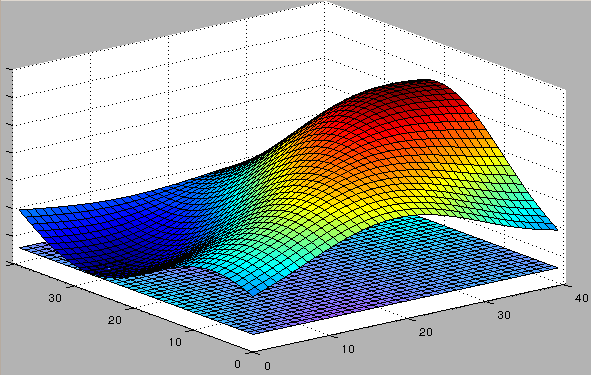
\includegraphics[width=0.45\textwidth]{lod-1.png}} 
  \subfigure[$LOD = 4$]{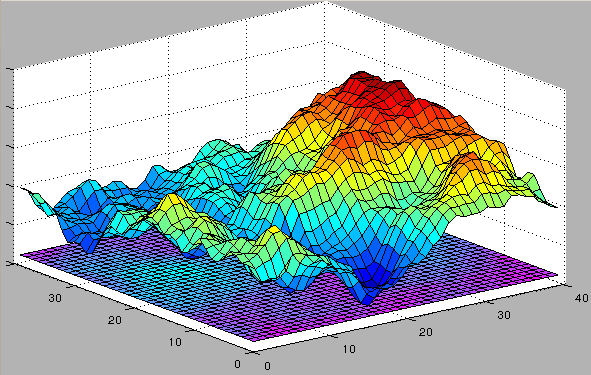
\includegraphics[width=0.45\textwidth]{lod-2.png}}
  \caption{Mapas gerados pelo algoritmo interno do simulador com $40$
    amostras (samples) e diferentes valores para o nível de detalhe
    (LOD).}
  \label{fig:lod}
\end{figure}

\subsection{Configurações da Simulação}

Três configurações podem ser alteradas na simulação: o algoritmo de
controle (\textbf{Control Algorithm}), o número de robôs
(\textbf{Robots}) e o passo de integração (\textbf{Time step}).

\begin{itemize}
\item \textbf{Control algorithm}: define qual arquivo externo será
  utilizado para controlar os robôs. Esse arquivo encontra-se no
  diretório \textbf{algorithms}, dentro do diretório raíz do
  \textit{ITVsim}.
\item \textbf{Robots}: o número de robôs da simulação.
\item \textbf{Time step}: o tempo de integração $\Delta t$ da simulação.
\end{itemize}

Para rodar a simulação, selecione um controlador da lista disponível,
o número de robôs e o tempo de integração. Logo após, clique no botão
\textbf{Simulate}. Se um terreno já existir, os robôs serão
inicializados sobre ele. Caso contrário, um novo terreno será
automaticamente criado de acordo com a sua configuração atual (Seção
\ref{sec:terrain}). Durante a simulação, todas as configurações serão
travadas nos seus respectivos valores, somente podendo ser alteradas
após o término da mesma. O botão \textbf{Stop} pode ser utilizado para
terminar a simulação em qualquer momento.

\subsection{Configurações do Renderizador}

As configurações do renderizador efetuam apenas mudanças estéticas no
visualizador. Existem duas opções: \textbf{Shading} e
\textbf{Lighting}, cada qual pode assumir três diferentes
valores. Tais configurações podem ser combinadas par a par,
totalizando 15 diferentes variedades estéticas. Algumas dessas são
mostradas na Figura \ref{fig:renderer}.

\begin{figure}[htpb]
  \centering
  \subfigure[Shading = Faceted]{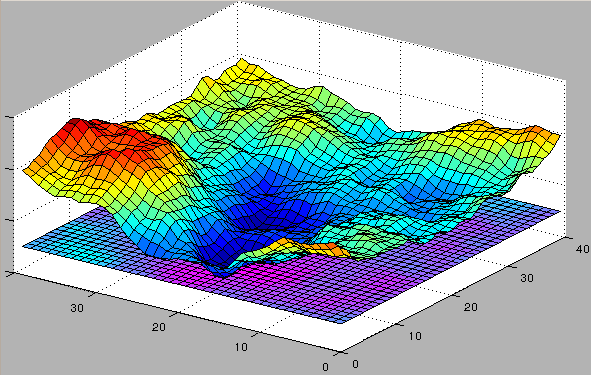
\includegraphics[width=0.45\textwidth]{renderer-1.png}} 
  \subfigure[Shading = Flat]{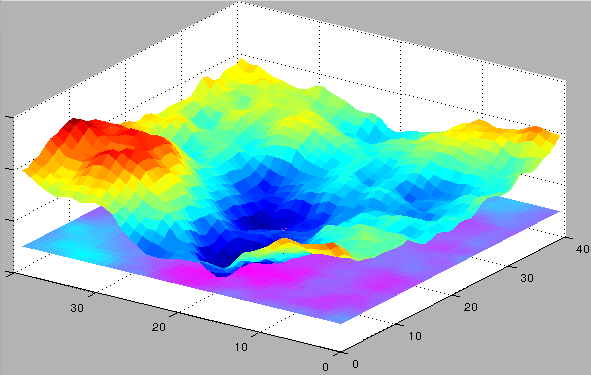
\includegraphics[width=0.45\textwidth]{renderer-2.png}}
  \subfigure[Shading = Interp]{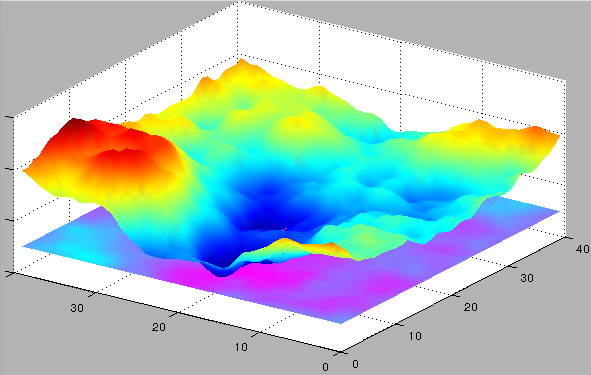
\includegraphics[width=0.45\textwidth]{renderer-3.png}}
  \subfigure[Lighting = Flat]{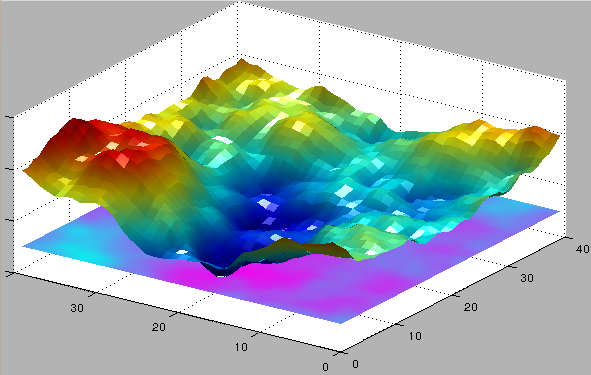
\includegraphics[width=0.45\textwidth]{renderer-4.png}}
  \subfigure[Lighting = Gouraud]{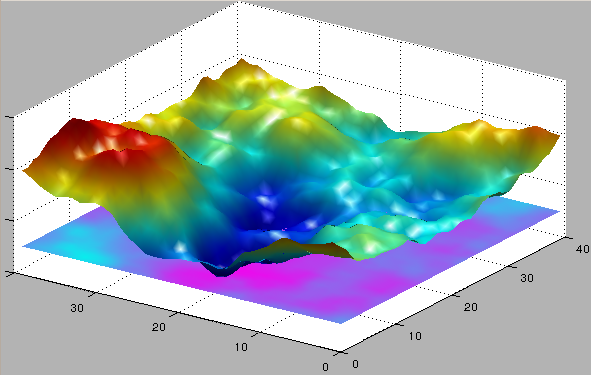
\includegraphics[width=0.45\textwidth]{renderer-5.png}}
  \subfigure[Lighting = Phong]{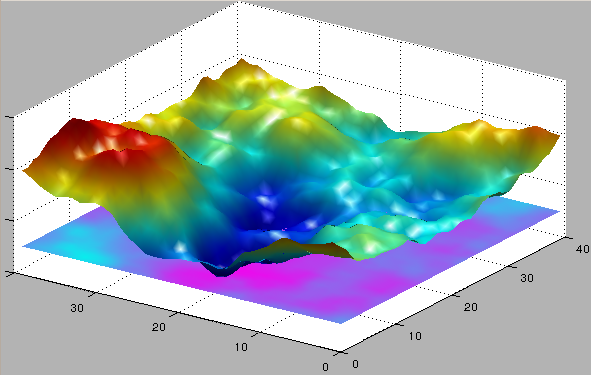
\includegraphics[width=0.45\textwidth]{renderer-6.png}}
  \caption{Diferentes configurações de interpolação de cores e modelos
    de iluminação do renderizador.}
  \label{fig:renderer}
\end{figure}

\begin{itemize}
\item \textbf{Shading}: controla a interpolação das cores na grade de vértices.
  \begin{itemize}
  \item \textbf{Flat}: colore cada face do terreno com uma única cor.
  \item \textbf{Faceted}: desenha linhas pretas conectando cada vértice.
  \item\textbf{Interp}: interpola linearmente as cores dos vértices em cada face.
  \end{itemize}

\item \textbf{Lighting}: controla a iluminação local da cena.
  \begin{itemize}
  \item \textbf{None}: desliga a iluminação.
  \item \textbf{Flat}: calcula a iluminação por face.
  \item \textbf{Gouraud}: calcula a iluminação por vértice.
  \item \textbf{Phong}: calcula a iluminação por pixel.
  \end{itemize}
\end{itemize}

\section{Desenvolvimento de Estratégias} 
\label{sec:strategies}

Para carregar uma nova estratégia no simulador basta criar uma nova
classe no diretório \textbf{algorithms} dentro do diretório raiz do
\textit{ITVsim}. Ao iniciar o simulador, os arquivos referentes a
classes do \textit{MATLAB} serão carregados e disponibilizados na
caixa \textbf{Control algorithm}. Para facilitar o desenvolvimento,
dois exemplos básicos estão inclusos: \textbf{RandomWalk.m} e
\textbf{Segregation.m}. No primeiro, os robôs navegam aleatoriamente,
enquanto no segundo eles são divididos de maneira autônoma em três
grupos contendo o mesmo número de robôs. Em ambos exemplos os robôs
tentam se manter em uma altura constante com relação ao solo.

\subsection{Classe Strategy}

Para definir uma estratégia é necessário estender a classe
\textbf{strategy}, através da qual o simulador efetua chamadas de alto
nível sem se preocupar com a implementação concreta. Em outras
palavras, a classe provê uma interface abstrata comum para todas as estratégias.

O construtor da classe recebe como entrada do simulador a grade de
vértices que representa o terreno. Portanto, qualquer nova estratégia
deve possuir esses mesmos parâmetros em seu construtor, sendo
obrigação da classe filha chamar o construtor de sua classe pai. Por
exemplo, o código mais básico para inicializar essa hierarquia é
apresentado logo abaixo, no qual a classe \textbf{NovaEstrategia} é
definida. Seu construtor recebe três matrizes bidimensionais contendo
as informações do terreno. Tais parâmetros seguem a especificação do
comando \textbf{surf} do \textit{MATLAB}.
\begin{lstlisting}
classdef NovaEstrategia < strategy
    methods
        function this = NovaEstrategia(x, y, z)
            this@strategy(x, y, z);
        end
end
\end{lstlisting}

Na implementação de uma estratégia, os métodos concretos mais
importantes são \textbf{initialize} e \textbf{control}. No primeiro, o
desenvolvedor pode especificar as posições e velocidades iniciais de
cada robô, além de escolher entre um modelo cinemático ou dinâmico de
controle. No segundo, o desenvolvedor tem acesso às posições e
velocidades de cada robô e deve determinar quais serão as respectivas
entradas de controle a partir dessas informações. A assinatura do
primeiro método é dada por 
\begin{lstlisting}
function [p, v, dynamics] = initialize(this, robots, limits)
\end{lstlisting}
no qual os valores de retorno $\mathbf{P}$ e $\mathbf{V}$ são matrizes
contendo as posições e velocidades iniciais de cada robô e
\textbf{dynamics} é uma variável booleana que define se as entradas de
controle devem ser interpretadas como acelerações ou velocidades, de
acordo com o valor \textbf{true} e \textbf{false},
respectivamente. Com relação aos parâmetros de entrada, \textbf{this}
é uma referência para uma instância da classe (o padrão de orientação
a objetos em \textit{MATLAB} requer essa declaração), \textbf{robots}
é o número de robôs e \textbf{limits} é um arranjo de duas posições
contendo o valor máximo do eixo X e Y.

A posição e a velocidade dos robôs é descrita por uma matrix $n \times
3$, sendo $n$ o número de robôs. Mais especificamente, seja
$\mathbf{p}_i = [x_i, y_i, z_i]^T$ o vetor de posição do robô
$i$. Dessa maneira, a matriz de posições conjunta $\mathbf{P}$ que deve
ser retornado pelo método \textbf{initialize} é dado por
\begin{equation}
  \mathbf{P} = 
 \begin{pmatrix}
    \mathbf{p}_1^T \cr
    \mathbf{p}_2^T \cr
    \vdots \cr
    \mathbf{p}_n^T
  \end{pmatrix}
  =
  \begin{pmatrix}
    x_1 & y_1 & z_1 \cr
    x_2 & y_2 & z_2 \cr
    \vdots & \vdots & \vdots \cr
    x_n & y_n & z_n
  \end{pmatrix},
\end{equation}
e o mesmo padrão é seguido para as velocidades, isto é, cada
coordenada em uma coluna da matriz. Essa descrição permite o uso da
função \textbf{bsxfun} do \textit{MATLAB}, que pode efetuar o cálculo
de distâncias entre todos os robôs com poucas linhas de código (veja o
exemplo no arquivo \textbf{Segregation.m}). Se um vetor vazio for
retornado para as posições, o simulador irá as inicializar com valores
aleatórios distribuídos uniformemente dentro das dimensões do
terreno. No caso das velocidades, elas serão inicializadas com a
matriz nula.

O método \textbf{control} possui a seguinte assinatura:
\begin{lstlisting}
function input = control(this, p, v)
\end{lstlisting}
onde $\mathbf{P}$ e $\mathbf{V}$ são as matrizes de posição e
velocidade já discutidas e a variável de retorno
\textbf{input} é uma matrix $n \times 3$ com as entradas de controle
dos robôs. A especificação dessa matriz segue a mesma descrição das
posições e velocidades, isto é, em cada linha são dadas as entradas de
controle de um robô específico e cada coluna é reservada para uma
dimensão específica.

\subsection{Exemplo Mínimo}

Abaixo segue o código fonte mínimo de uma estratégia que mantém os
robôs parados no solo. Ambas as matrizes de posições e velocidades são
inicializadas com valores vazios, o que delega a responsabilidade de
posicionar os robôs no terreno para o simulador. Também, um modelo de
controle dinâmico é selecionado, isto é, os valores de retorno do
método \textbf{control} serão interpretados como acelerações. Esse
método apenas cria uma matriz nula como entrada de controle e a
retorna para o simulador.

\begin{lstlisting}
classdef NovaEstrategia < strategy
    properties (SetAccess = private)
        robots
    end
    
    methods
        function this = NovaEstrategia(x, y, z)
            this@strategy(x, y, z);
        end
        
        function [p, v, dynamics] = initialize(this, r, wl)
            p = []; v = []; 
            dynamics = true; 
            this.robots = r;
        end
        
        function input = control(this, p, v)
            input = zeros(this.robots, 3);
        end
    end
end
\end{lstlisting}

\end{document}